\documentclass[tikz,border=2pt]{standalone}
\usepackage[T1]{fontenc}
\usepackage{mathptmx}
\usepackage{amsmath}
\usetikzlibrary{arrows.meta,positioning,calc,fit}

\tikzset{
  every node/.style={font=\fontsize{7.2}{8.4}\selectfont, inner sep=2.5pt, align=center},
  blk/.style={draw=black, line width=0.5pt, fill=white, minimum height=1.4cm},
  cal/.style={draw=black, line width=0.5pt, fill=black!7, minimum height=1.4cm},
  ar/.style={-{Stealth[length=3.4pt,width=2.8pt]}, line width=0.5pt},
  bi/.style={{Stealth[length=3.4pt,width=2.8pt]}-{Stealth[length=3.4pt,width=2.8pt]}, line width=0.5pt},
  lb/.style={font=\fontsize{6.3}{7}\selectfont, inner sep=1pt},
}
\newcommand{\sm}{\fontsize{6.3}{7}\selectfont}

\begin{document}
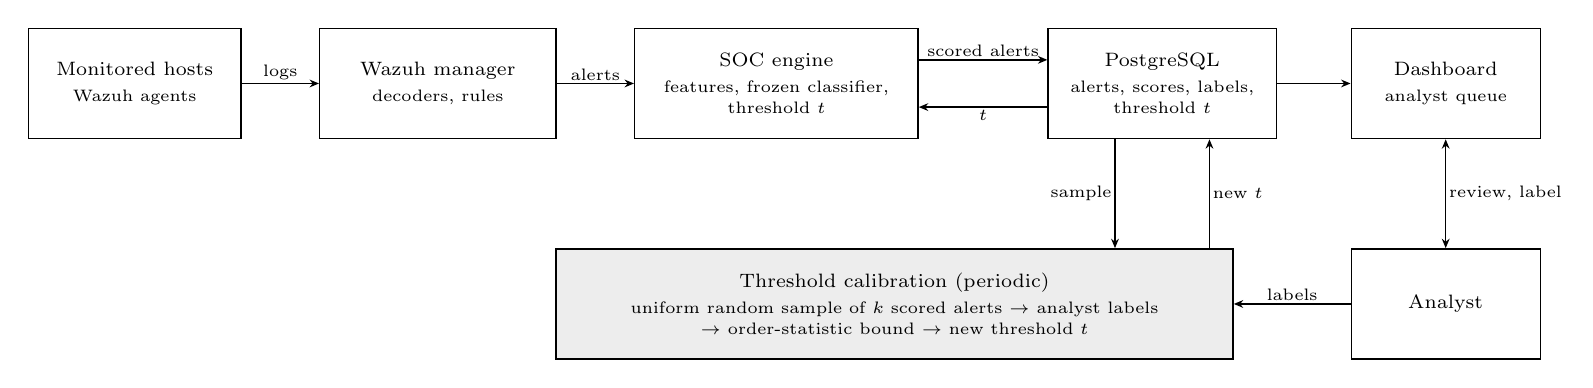
\begin{tikzpicture}[x=1cm,y=1cm]
% ---- top row: data path
\node[blk, minimum width=2.7cm] (host) at (1.35,3.2) {Monitored hosts\\[1pt]\sm Wazuh agents};
\node[blk, minimum width=3.0cm] (mgr)  at (5.2,3.2) {Wazuh manager\\[1pt]\sm decoders, rules};
\node[blk, minimum width=3.6cm] (eng)  at (9.5,3.2) {SOC engine\\[1pt]\sm features, frozen classifier,\\[-1pt]\sm threshold $t$};
\node[blk, minimum width=2.9cm] (db)   at (14.4,3.2) {PostgreSQL\\[1pt]\sm alerts, scores, labels,\\[-1pt]\sm threshold $t$};
\node[blk, minimum width=2.4cm] (dash) at (18.0,3.2) {Dashboard\\[1pt]\sm analyst queue};
\draw[ar] (host) -- node[lb, above]{logs} (mgr);
\draw[ar] (mgr) -- node[lb, above]{alerts} (eng);
\draw[ar] ($(eng.east)+(0,0.3)$) -- node[lb, above]{scored alerts} ($(db.west)+(0,0.3)$);
\draw[ar] ($(db.west)+(0,-0.3)$) -- node[lb, below]{$t$} ($(eng.east)+(0,-0.3)$);
\draw[ar] (db) -- (dash);
% ---- bottom row: calibration loop
\node[cal, minimum width=8.6cm] (calib) at (11.0,0.4) {Threshold calibration (periodic)\\[1pt]\sm uniform random sample of $k$ scored alerts $\rightarrow$ analyst labels\\[-1pt]\sm $\rightarrow$ order-statistic bound $\rightarrow$ new threshold $t$};
\node[blk, minimum width=2.4cm] (ana) at (18.0,0.4) {Analyst};
\coordinate (s1) at ($(db.south)+(-0.6,0)$);
\coordinate (s2) at ($(db.south)+(0.6,0)$);
\draw[ar] (s1) -- node[lb, left]{sample} (s1 |- calib.north);
\draw[ar] (s2 |- calib.north) -- node[lb, right]{new $t$} (s2);
\draw[bi] (dash) -- node[lb, right]{review, label} (ana);
\draw[ar] (ana) -- node[lb, above]{labels} (calib);
\end{tikzpicture}
\end{document}
